\documentclass{report}
% package para el simbolo dotminus
\usepackage{amsmath}

% macro para dotminus
\makeatletter
\newcommand{\dotminus}{\mathbin{\text{\@dotminus}}}
\newcommand{\@dotminus}{%
  \ooalign{\hidewidth\raise1ex\hbox{.}\hidewidth\cr$\m@th-$\cr}%
}
\makeatother


\input{preamble}
\input{macros}
\input{letterfonts}

\title{\Huge{Guia Practica 1}\\LyC 2024 2C}
\author{\huge{Pablo Mercado}}
\date{}

\begin{document}

\maketitle
\newpage% or \cleardoublepage
% \pdfbookmark[<level>]{<title>}{<dest>}
\pdfbookmark[section]{\contentsname}{toc}
\tableofcontents
\pagebreak

\chapter{}

% Add "pregunta1" to the TOC
\addcontentsline{toc}{section}{Ejercicio 1}
\qs{pregunta1}{
	$\textbf{Ejercicio 1. }$  Mostrar que,  dado un k fijo, la función constante $f(x)=k$ puede defnirse usando
	las funciones iniciales y composición $(sin$ usar recursión primitiva).
}
\sol Cualquier $ k \in \mathbb{N}$ puede ser construido aplicando sucesivamente la funcion $s(x)$ a la funcion $n(x)$.
\begin{align}
	f(x)= s_k (x) = \underbrace{s(s(\ldots s(n(x))\ldots))}_{k\ \text{veces}}
\end{align}

Ya que $s(n(x))$ es composicion de funciones primitivas, es primitiva recursiva.
Razonando de forma inductiva, cada vez que aplicamos $s(x)$ a un cierto $s_{k-1} (x)$, obtenemos un $s_k (x)$ que de nuevo, por composicion, es primitiva recursiva.




\addcontentsline{toc}{section}{Ejercicio 2}
\qs{}{

	Ejercicio 2. Probar que las signicntes funciones son primitivas recursivas, mostrando que pueden
	obtenerse a partir des funciones iniciales usando composición y/o recursion primitiva:

	$\begin{aligned}
			\\
			 & f_1(x,y)=x+y\quad f_2(x,y)=x\cdot y\quad f_3(x,y)=x^y\quad f_4(x,y)=\underbrace{x^{x^{x^{\cdot^{\cdot^{\cdot^{\cdot^{x}}}}}}}}_{y\ \text{veces}} \\
			\\
			 & g_1(x)=x \dotminus 1\quad g_2(x,y)=x \dotminus y\quad g_3(x,y)=\max\{x,y\}\quad g_4(x,y)=\min\{x,y\}                                             \\
			\\
			 & Observaciones:\text{Se asume que }f_4(x,0)=1.\quad x\dotminus y=\begin{cases}x-y & \text{si }y\leq x \\
             0   & \text{si }y>x\end{cases}
		\end{aligned}$
}

\sol $f_1(x,y) = x+y$
\begin{align*}
	f_1(x,0) & = 0 = n(x)                                                 \\
	f_1(x,y) & = \underbrace{((\ldots((0+1)+1)\ldots+1)+1)+1}_{y \ veces} \\
	f_1(x,y) & = f_1(x,y-1)+1                                             \\
	         & = s(f_1(x,y-1))                                            \\
\end{align*}

Pero para que cierre la aridad con el esquema de recursion primitiva, debemos encontrar una funcion g tal que:
$f_1(x,y) = g(f(x,y-1),x,y-1)$, esto se arregla tomando $g(x,y,z) = s(u_1^3(x,y,z))$
Entonces nos queda:
\begin{align}
	f_1(x,y) = g(f(x,y-1),x,y-1) = s(u_1^3(f(x,y-1),x,y-1))
\end{align}

\sol $f_{2}(x,y)=x.y$
\begin{align*}
	 & f_{2}(x,0)=n(x)                                                   \\
	 & f_2(x,y)=f_2(x,y-1)+x=f_1(f_2(x,y-1),x)                           \\
	 & f_{2}(x,y)= f1(u_1^3(f_2(x,y-1),x,y-1),\ u_2^3(f_2(x,y-1),x,y-1)) \\
	 & f_{2}(x,y)= g(f_2(x,y-1),x,y-1)
\end{align*}

Con $g(x,y,z) = f_1(u_1^3(x,y,z),u_2^3(x,y,z))$, ya que $g$ se obtiene por coposicion de funciones PR, entonces tambien es PR.

~

\sol $f_{3}(x,y)=x^{y}$
\begin{align*}
	 & f_{3}(x,0)=1                                                                  \\
	 & f_{3}(x,y)=f_{3}(x,y-1).x=f_{2}(f_{3}(x,y-1),x)                               \\
	 & f_{3}(x,y)=f_{2}(u_{1}^{3}(f_{3}(x,y-1),x,y-1),u_{2}^{3}(f_{3}(x,y-1),x,y-1)) \\
	 & f_{3}(x,y)= g(f_3(x,y-1),x,y-1)
\end{align*}

Con $g(x,y,z) = f_2(u_1^3(x,y,z),u_2^3(x,y,z))$, ya que $g$ se obtiene por coposicion de funciones PR, entonces tambien es PR.

~

\sol
$f_4(x,y)=\underbrace{x^{x^{x^{\cdot^{\cdot^{\cdot^{\cdot^{x}}}}}}}}_{y\ \text{veces}}$
\begin{align*}
	 & f_{4}(x,0)=1                                                                  \\
	 & f_{4}(x,y)=f_{4}(x,y-1)^{x}=f_{3}(f_{4}(x,y-1),x)                             \\
	 & f_{4}(x,y)=f_{3}(u_{1}^{3}(f_{4}(x,y-1),x,y-1),u_{2}^{3}(f_{4}(x,y-1),x,y-1))
\end{align*}

Con $g(x,y,z) = f_3(u_1^3(x,y,z),u_2^3(x,y,z))$, ya que $g$ se obtiene por coposicion de funciones PR, entonces tambien es PR.

~

\sol
$g_1(x)=x \dotminus 1$
\begin{align*}
	 & g_{1}(0)=n(x) \\&g_{1}(x)=u_{2}^{2}(g_{1}(x),x-1)
\end{align*}

~

\sol
$g_2(x,y)=x \dotminus y$
\begin{align*}
	 & g_{2}(x,0)=u_{1}^{1}(x)                         \\
	 & g_{2}(x,y)=g_{2}(x,y-1)-1=g_{1}(g_{2}(x,y-1))   \\
	 & g_{2}(x,y)=g_{1}(u_{1}^{3}(g_{2}(x,y-1),x,y-1)) \\
	 & g_{2}(x,y)=g(g_{2}(x,y-1),x,y-1)
\end{align*}

Con $g(x,y,z) = g_2(u_1^3(x,y,z))$, ya que $g$ se obtiene por coposicion de funciones PR, entonces tambien es PR.

~

\sol
$g_3(x,y)=\max\{x,y\}$
\begin{align*}
	 & \max\{x,y\}=(x\leqslant y).y+\alpha(x\leqslant y).x                                                                \\
	 & \max\{x,y\}=f_{2}((x\leqslant y),y)+f_{2}(\alpha(x\leqslant y),y)                                                  \\
	 & \max\{x,y\}=f_{1}(\underbrace{f_{2}((x\leqslant y),y)}_{h_{1}},\underbrace{f_{2}(\alpha(x\leqslant y),y)}_{h_{2}})
\end{align*}

Las funciones $\alpha$ (negacion) y $\leq$ son las definidas en la clase teorica numero 2.
Se puede probar por composicion que $h_1$ y $h_2$ son PR. Por lo tanto queda demostrado por composicion que $g_3$ tambien es PR.

~

\sol
$g_4(x,y)=\min\{x,y\}$
\begin{align*}
	 & \min\{x,y\}=(x\leqslant y).x+\alpha(x\leqslant y).y                                                                \\
	 & \min\{x,y\}=f_{2}((x\leqslant y).x)+f_{2}(\alpha(x\leqslant y),y)                                                  \\
	 & \min\{x,y\}=f_{1}(\underbrace{f_{2}((x\leqslant y),y)}_{h_{1}},\underbrace{f_{2}(\alpha(x\leqslant y),y)}_{h_{2}})
\end{align*}

Las funciones $\alpha$ (negacion) y $\leq$ son las definidas en la clase teorica numero 2.
Se puede probar por composicion que $h_1$ y $h_2$ son PR. Por lo tanto queda demostrado por composicion que $g_3$ tambien es PR.






\qs{}{
Ejercicio 3. Sea $\mathcal{C}_i$ la clase de funciones iniciales, es decir, aquella que contiene a:\\\\
$n( x) = 0$ \ \ \ \ $s( x) = x+ 1$ \ \ \ \
$u_i^n(x_1,\ldots,x_n)=x_i$ para cada $n\in\mathbb{N}$ e $i\in\{1,\ldots,n\}$\\

$\begin{aligned}&\text{y sea }\mathcal{C}_c\text{ la (mínima) clase que extiende a }\mathcal{C}_i\text{ y se encuentra cerrada por composición, i.e., si}\\&f,g_1,\ldots g_m\text{ están en }\mathcal{C}_c,\text{ entonces }h(x_1,\ldots,x_n)=f(g_1(x_1,\ldots,x_n),\ldots,g_m(x_1,\ldots,x_n))\text{ también}\\&\text{lo está.}\end{aligned}$
\\\\a. Demostrar que para toda $f: \mathbb{N} ^n\to \mathbb{N} , f\text{ est\' {a} en }\mathcal{C} _c$ sii existe $k\geq0$ tal que, o bien sucede
$f(x_1,\ldots,x_n)=k$, o bien para algún $i$ fijo, se tiene $f(x_1,\ldots,x_n)=x_i+k.$
\\\\b. Mostrar que existe una función primitiva recursiva que no está en $\mathcal{C}_c.$
}

\addcontentsline{toc}{section}{Ejercicio 3}
\sol a)

($\rightarrow$)

Vamos a usar induccion estructural

Casos Base:
Veamos que se cumple para las funciones iniciales
\begin{align*}
	 & n(x)=0,\ \ k=0                   \\
	 & s(x)=x+1,\ \ k=1                 \\
	 & u_i^n(x_1,...,x_n)=x_i+0,\ \ k=0
\end{align*}
\\
Paso inductivo:\\
Sea $f \in \mathcal{C}$, $f(x_1, \ldots, x_n) = h(g_1(x1, \ldots, x_n), \ldots, g_n(x1, \ldots, x_n))$.
Veamos que o bien $f(x_1, \ldots, x_n) = k$, o bien  $f(x_1, \ldots, x_n) = x_i + k$
\\\\
Las funciones que componen a h, cumplen con la HI. Por lo tanto, separemos en casos:
\\\\
Caso $h(x1, \ldots, x_n) = k$: Entonces tenemos que $f(x1, \ldots, x_n) = k = k'$, ya esta!
\\\\
Caso $h(x1, \ldots, x_n) = x_i + k'$: Entonces tenemos que $f(x1, \ldots, x_n) = g_i(x1, \ldots, x_n)$.

Ahora tenemos 2 sub-casos mas:

Caso $g_i(x1, \ldots, x_n) = k''$:  $f(x1, \ldots, x_n) = k' + k'' = k$

Caso $g_i(x1, \ldots, x_n) = x_j + k''$: $f(x1, \ldots, x_n) = x_j + k'' + k' = x_j + k$
\\
En ambos casos, vemos que se cumple lo que queriamos.
\\\\

($\leftarrow$)\\
Ya vimos que la funcion $h_k(x) = k$, puede ser definida por composicion y recursion a partir de
las funciones iniciales, entonces $h_k \in \mathcal{C}$.
Entonces $f(x_1 , \ldots , x_n) = h_k(u_1^n(x_1 , \ldots , x_n)) = k$, xlt $f \in \mathcal{C}$
\\\\
Se puede defnir la funcion $s_k(x) = x + k$ usando sucesivamente la funcion $s$, por composicion $s_k \in \mathcal{C}$.
Xlt $f(x_1, ... , x_n) = x_i  + k = s_k(u_i^n(x_1, ... , x_n))$. Y esta ultima al ser composicion de funciones de
$\mathcal{C}$, nos asegura que f tambien esta en $\mathcal{C}$.


\qs{}{
$\textbf{Ejercicio 4.}\text{Llamamos}\  predicado$ a cualquier función $p:\mathbb{N}^n\to\{0,1\}$, escribimos $p(a_1,\ldots,a_n)$ en lugar de $p(a_1,\ldots,a_n)=1$ y decimos, informalmente, en ese caso, que “$p(a_1,\ldots,a_n)$ es verdadero" Mostrar que los predicados $\leq,\geq,=,\neq,<$y$> : \mathbb{N} ^2\to \{ 0, 1\} \text{ est\' {a}n\ en\ cualquier\ clase\ }PRC.$
}
\addcontentsline{toc}{section}{Ejercicio 4}
\sol \\

$\begin{aligned}&\bullet\leq(x,y)=\alpha(x-y)\\&\bullet\geq(x,y)=\alpha(y-x)\\&\bullet=(x,y)=(x\leq y).(y\leq x)\\&\bullet\neq(x,y)=\alpha(x=y)\\&\bullet<(x,y)=\alpha(x\geq y)\\&\bullet>(x,y)=\alpha(x\leq y)\end{aligned}$

~


Si una funcion f esta en cualquier clase PRC, entonces esta en la interseccion de todas las clases PRC, por el teorema visto en clases, podemos decir que
ser funcion primitiva recursiva es condicion necesaria y suficiente para esto.
En el ejericio 2 vimos que la funcion de multiplicacion, resta de naturales y la suma son primitivas recursivas. Probemos que $\alpha(x)$ es primitiva recursiva.

\[
	\begin{aligned}
		\alpha:N\rightarrow\{0,1\} \\
		\alpha(x)=\begin{cases}
			          1 & \text{si } x=0    \\
			          0 & \text{si } x\neq0
		          \end{cases}
	\end{aligned}
\]

Ahora vamos a definir $\alpha(x)$ por recursion primitiva.\\

$$\begin{aligned}
		\alpha(0)   & =s(n(x))=1                                                      \\
		\alpha(x+1) & =g(\alpha(x-1),x)=0 \ \ \ \ \text{con\ } g(x,y) = n(u_2^2(x,y)) \\
		\alpha(x+1) & =n(u_{2}^{2}(\alpha(x),x))=0
	\end{aligned}$$\\

Entonces $\alpha(x)$ es primitiva recursiva.
Las funciones que describimos arriba estan formadas por composicion entre funciones primitivas recursivas, por lo tanto son primitivas recursivas.\\





\qs{}{
\addcontentsline{toc}{section}{Ejercicio 5}
Ejercicio 5. Sea $\mathcal{C}$ una clase $PRC$, sean $f_1,\ldots,f_k,g:\mathbb{N}^n\to\mathbb{N}$ funciones en $\mathcal{C}$ y sean también $p_1,\ldots,p_k:\mathbb{N}^n\to\{0,1\}$ predicados disjuntos en $\mathcal{C}$ (i.e., no sucede $p_i(a_1,\ldots,a_n)=p_j(a_1,\ldots,a_n)=$ 1 con $i\neq j\text{ para ning\' {u}n}( a_1, \ldots , a_n) \in \mathbb{N} ^n) .$ Mostrar que también está en $\mathcal{C} \text{ cualquier funcion} \ h$ que cumpla:

\begin{align}
	h(x_1,\dots,x_n)=\left\{\begin{array}{cl}f_1(x_1,\dots,x_n)&\text{si }p_1(x_1,\dots,x_n)\\\vdots\\f_k(x_1,\dots,x_n)&\text{si }p_k(x_1,\dots,x_n)\\g(x_1,\dots,x_n)&\text{si no}\end{array}\right.
\end{align}
Observar que $h$ queda completamente determinada por el esquema.
}
\sol \\
$$\begin{aligned}
		h(x_1,...,x_n) = & f_{1}(x_{1},...,x_{n}).p_{1}(x_{1},...,x_{n})+                           \\
		                 & f_2(x_1,...,x_n).p_2(x_1,...,x_n)+                                       \\
		                 & f_k(x_1,...,x_n).p_k(x_1,...,x_n)+                                       \\
		                 & \vdots                                                                   \\
		                 & g(x_1,\ldots,x_n).\alpha(p_1(x_1,\ldots,x_n)+\ldots+p_k(x_1,\ldots,x_n))
	\end{aligned}$$
\\
Notemos que $g(x_1,\ldots,x_n).\alpha(p_1(x_1,\ldots,x_n)+\ldots+p_k(x_1,\ldots,x_n))$ toma el valor 1, sii todos los predicados valen 0 a la vez.

Sabemos que toda clase PRC contiene a las funciones inicales. En el ejericio 2, vimos que las funciones $f_1(x,y) = x+y$ y $f_2(x,y) = x.y$ son primitivas recursivas, por teorema, sabemos que esta en cualquier clase PRC.
Para que h este en $\mathcal{C}$ tiene que poder obtenerse a partir de otras en $\mathcal{C}$ mediante recursion primitiva o composicion.


\clm{}{}{
	$f_i(x_1,...,x_n).p_i(x_1,...,x_n)\in \mathcal{C}$
}
\begin{myproof}
	Trivial, ya que $f_2(x,y) = x.y \in \mathcal{C}$ por ser pr.
\end{myproof}


\clm{}{}{
	$a_n(x_1, \ldots, x_n) =x_1+ \ldots+ x_n$ es primitiva recursiva.
}
\begin{myproof}
	Notemos que la funcion $a_n$  puede ser obtenida aplicando la funcion suma ($f_1$) sucesivamente (composicion) de esta manera:
	$a_n(x_1,\ldots,x_n)=f_1(\ldots(f_1(f_1(x_1,x_2),x_3))\ldots,x_n)$. Entoces $ a_n(x_1,\ldots,x_n)\in \mathcal{C}$. Mas generalmente, culaquier funcion que sume todos sus parametros
	es primitiva recursiva.
\end{myproof}


\clm{}{}{
	$g(x_1, \ldots , x_n) = \alpha(p_1(x_1,\ldots,x_n)+\ldots+p_k(x_1,\ldots,x_n)) \in \mathcal{C}$
}
\begin{myproof}
	$g(x_1, \ldots , x_n) = \alpha(a_n(p_1(x_1, \ldots , x_n), \ldots, p_n(x_1, \ldots , x_n))) = g'(p_1(x_1, \ldots , x_n), \ldots, p_n(x_1, \ldots , x_n))$
	\\Con $h'(x_1, \ldots , x_n) = \alpha \circ a_n (x_1, \ldots , x_n)$
\end{myproof}

\clm{}{}{

	$$\begin{aligned}
			h(x_1,...,x_n) = & f_{1}(x_{1},...,x_{n}).p_{1}(x_{1},...,x_{n})+                                           \\
			                 & f_2(x_1,...,x_n).p_2(x_1,...,x_n)+                                                       \\
			                 & f_k(x_1,...,x_n).p_k(x_1,...,x_n)+                                                       \\
			                 & \vdots                                                                                   \\
			                 & g(x_1,\ldots,x_n).\alpha(p_1(x_1,\ldots,x_n)+\ldots+p_k(x_1,\ldots,x_n)) \in \mathcal{C}
		\end{aligned}$$
}

\begin{myproof}
	Sean: \\ $f_i'(x_1,\ldots,x_n) = f_i(x_1,\ldots,x_n).p_i(x_1,\ldots,x_n) \in \mathcal{C} , \forall i: 1 \ldots k$
	\\ $g'(x_1,\ldots,x_n) = g(x_1,\ldots,x_n).\alpha(p_1(x_1,\ldots,x_n)+\ldots+p_k(x_1,\ldots,x_n)) \in \mathcal{C}$
	\\\\ Escribamos a $h$ como composicion de funciones en $\mathcal{C}$ \\
	$h(x_1,\ldots,x_n) = a_{k+1}(f_1'(x_1,\ldots,x_n), \ldots,f_k'(x_1,\ldots,x_n), g'(x_1,\ldots,x_n))$. \\$\therefore h \in \mathcal{C}$.


\end{myproof}


\qs{}{
$\textbf{Ejercicio 6.}$
a) Demostrar que el predicado $\text{par}(x)=\begin{cases}1&\text{ si }x\text{ es par}\\0&\text{ si no}\end{cases}$ esta en toda clase PRC.
\\
b. Demostrar que la función $f( x) = \lfloor x/ 2\rfloor \text{ est\'{a}  en toda clase }PRC.$
\\\\c. Sea $\mathcal{C}$ una clase $PRC$, y sean $f:\mathbb{N}^n\to\mathbb{N}$ y $g_1,g_2:\mathbb{N}^{n+2}\to\mathbb{N}$ funciones en $\mathcal{C}$. Mostrar que
también está en $\mathcal{C}$ cualquier $h$ que cumpla:
$$h(x_1,\dots,x_n,t)=\left\{\begin{array}{ll}f(x_1,\dots,x_n)&\:\textrm{si}\:t=0\\g_1(x_1,\dots,x_n,k,h(x_1,\dots,x_n,t-1))&\:\textrm{si}\:t=2\cdot k+1\\g_2(x_1,\dots,x_n,k,h(x_1,\dots,x_n,t-1))&\:\textrm{si}\:t=2\cdot k+2\end{array}\right.$$
Observar que $h$ queda completamente determinada por este esquema.
}
\addcontentsline{toc}{section}{Ejercicio 6}
\sol a)
\mprop{}{
	$\text{par}(x)=\begin{cases}1&\text{ si }x\text{ es par}\\0&\text{ si no}\end{cases}$ esta en toda clase PRC.
}
\begin{myproof}
	Sabemos que estar en toda clase PRC es equivalente a ser funcion primitiva recursiva, veamos que par$(x)$ cumple esto.

	$$\begin{aligned}
			 & par(0)=1=s(n(x))                                               \\
			 & par(x+1)=\alpha(par(x))=\alpha(u_{1}^{2}(Par(x),x))            \\
			 & par(x+1)=g(Par(x),x) \ \ \ \ \text{con} \  g=\alpha\circ u^{2}
		\end{aligned}$$
	Ya que pudimos definir a la funcion par por recursion primitiva, entonces par es primitiva recursiva. $\therefore$ par esta en toda clase PRC.
\end{myproof}


\sol b)
\mprop{}{
$f( x) = \lfloor x/ 2\rfloor \text{ est\'{a}  en toda clase }PRC.$
}
\begin{myproof}
	\nt{
		$$\begin{array}{r|r|r|r|r|r|r|r|r|r|r|r}x&0&1&2&3&4&5&6&7&8&9&10\\\hline\lfloor\frac x2\rfloor&0&0&1&1&2&2&3&3&4&4&5\end{array}$$
		$$f(x)=\lfloor\frac{x}{2}\rfloor=\begin{cases}0&\mathrm{si~}x=0\\f(x-1)+\underbrace{\alpha(\mathrm{par}(x))}_{\mathrm{impar}(x)}&\mathrm{c.c}\end{cases}$$
	}
	$$\begin{aligned}
			 & f(0)=0=n(x)                                                                   \\
			 & f(x+1)=f(x)+\text{impar}(x)                                                   \\
			 & f(x+1)=f_{1}(f(x),\text{impar}(x))                                            \\
			 & f(x+1)=g(f(x),x) \ \ \ \ \text{con } g(x)=f_{1}(u_{1}^{1}(x),\text{impar}(x))
		\end{aligned}$$\\Entonces f es primitiva recursiva y por lo tanto esta en toda clase PRC.
\end{myproof}



\sol c)
\mprop{}{
	$h$ puede ser re-escrito como:
	$$h(x_1,\dots,x_n,t)=\left\{
		\begin{array}{ll}
			f(x_1,\dots,x_n)                                                   & \:\textrm{si}\:t=0                \\
			g_1(x_1,\dots,x_n, \lfloor\frac{t-1}2\rfloor,h(x_1,\dots,x_n,t-1)) & \:\textrm{si}\:t \text{ es impar} \\
			g_2(x_1,\dots,x_n,\lfloor\frac{t-1}2\rfloor,h(x_1,\dots,x_n,t-1))  & \:\textrm{si}\:t \text{ es par}
		\end{array}\right.$$
}
\begin{myproof}
	\begin{align*}
		 & \bullet \text{si } t = 2k + 1 \text{ es impar, entonces } \left\lfloor \frac{(2k+1)-1}{2} \right\rfloor = k \\
		 & \bullet \text{si } t = 2k + 2 \text{ es par, entonces } \left\lfloor \frac{(2k+2)-1}{2} \right\rfloor = k   \\
	\end{align*}De esto podemos deducir que $\left\lfloor \frac{t-1}{2} \right\rfloor = k$
\end{myproof}
\mprop{}{
	$h$ puede ser obtenido por recursion primitiva y por lo tanto esta en $\mathcal{C}$:
	$$h(x_1,\dots,x_n,t)=\left\{
		\begin{array}{ll}
			f(x_1,\dots,x_n)                          & \:\textrm{si}\:t=0 \\
			g(h(x_1,\dots,x_n,t-1),x_1,\dots,x_n,t-1) & \: \text{ c.c}
		\end{array}\right.$$
}
\begin{myproof}
	Nos gustaria encontar una funcion $g$ $\in \mathcal{C}$, tal que: $$g_i(x_1,\ldots,x_n,\lfloor\frac{t-1}2\rfloor,h(x_1,\ldots,x_n,t-1))=g(h(x_1,\ldots,x_n,t-1),x_1,\ldots,x_n,t-1)$$
	Esto lo podemos hacer cambiando de lugar los parametros y "desenvolviendo" el parametro t-1, para que quede solo. Definamos la funcion g.
	$$g(u_{n+2}^{n+2}(x_1,\ldots,x_{n+2}),u_1^{n+2}(x_1,\ldots,x_{n+2}),\ldots,u_{n}^{n+2}(x_1,\ldots,x_{n+2}),e(x_1,\ldots,x_{n+2}))$$Donde:
	$$\begin{aligned}&d(\mathrm{x})=2.\mathrm{x}+\mathrm{impar}(\mathrm{x})\\&e(x_1,\ldots,x_{n+2})=d(u_{n+1}^{n+2}(x_1,\ldots,x_{n+2}))\end{aligned}$$Se puede probar que $d$ y $e$ son funciones primitivas recursivas, por lo tanto, estan en $\mathcal{C}$.
	La funcion $d$ es la que "desenvuelve" el parametro t-1 de la funcion $\lfloor\frac{t}2\rfloor$. Entonces $g$ esta correctamente definida por composicion de funciones en $\mathcal{C}$.
	$\therefore h \in \mathcal{C}$.
\end{myproof}




\qs{}{
	$\begin{aligned}&\textbf{Ejercicio 7.} \text{Sea C una clase PRC y sea }p:\mathbb{N}^{n+1}\to\{0,1\}\text{ un predicado en }\mathcal{C}.\text{ Mostrar que}\\&\text{también están en }\mathcal{C}\text{ las siguientes funciones:}\end{aligned}$
	$\begin{aligned}
			\mathrm{cantidad}_p(x_1,\ldots,x_n,y,z)     & =|\{t\mid y\leq t\leq z\wedge p(x_1,\ldots,x_n,t)\}|                                                                          \\
			\mathrm{todos}_{p}(x_{1},\ldots,x_{n},y,z)  & =\left\{\begin{array}{ll}1&\text{ si }(\forall t:y\leq t\leq z)p(x_1,\dots,x_n,t)\\0&\text{ si no}\end{array}\right.          \\
			\mathrm{alguno}_{p}(x_{1},\ldots,x_{n},y,z) & =\left\{\begin{array}{ll}1&\text{ si }(\exists t:y\leq t\leq z)p(x_1,\dots,x_n,t)\\0&\text{ si no}\end{array}\right.          \\
			\mathrm{minimo}_{p}(x_{1},\ldots,x_{n},y,z) & =\begin{cases}\min\{t\mid y\leq t\leq z\land p(x_1,\dots,x_n,t)\}&\text{si existe tal t}\\0&\text{si no}\end{cases}           \\
			\mathrm{maximo}_{p}(x_{1},\ldots,x_{n},y,z) & =\begin{cases}\max\{t\mid y\leq t\leq z\land p(x_1,\dots,x_n,t)\}&\text{si existe tal t}\\0&\text{si no}\end{cases}           \\
			\mathrm{unico}_p(x_1,\ldots,x_n,y,z)        & =\left\{\begin{array}{ll}u&\text{si} \{u\}=\{t\mid y\le t\le z\wedge p(x_1,\dots,x_n,t)\}\\z+1&\text{si no}\end{array}\right.
		\end{aligned}$
	\\
	Observacion: pueden usarse los operadores acotados (min, $\sum$, $\forall$, $\exists$) vistos en la teorica.
}

~

\sol $\mathrm{cantidad}_p(x_1,\ldots,x_n,y,z) =|\{t\mid y\leq t\leq z\wedge p(x_1,\ldots,x_n,t)\}|$

$$\begin{aligned}
	\text{cantidad}_p(x_1,\ldots,x_n,y,z)=\sum_{t=y}^z p(x_1,...,x_n,t)
\end{aligned}$$

\sol $\mathrm{todos}_{p}(x_{1},\ldots,x_{n},y,z)   =\left\{\begin{array}{ll}1&\text{ si }(\forall t:y\leq t\leq z)p(x_1,\dots,x_n,t)\\0\text{ si no}\end{array}\right. $ 
$$\mathrm{todos}_{p}(x_{1},\ldots,x_{n},y,z)=(\forall t)_{\leq z}(y\leq t\lor P(x_1,\ldots,x_n,t))$$

\sol $\mathrm{alguno}_{p}(x_{1},\ldots,x_{n},y,z) =\left\{\begin{array}{ll}1\text{ si }(\exists t:y\leq t\leq z)p(x_1,\dots,x_n,t)\\0\text{ si no}\end{array}\right. $ 
$$\mathrm{alguno}_{p}(x_{1},\ldots,x_{n},y,z) = 1 \leq \text{cantidad}_p(x_{1},\ldots,x_{n},y,z) $$

\sol $\mathrm{minimo}_{p}(x_{1},\ldots,x_{n},y,z) =\begin{cases}\min\{t\mid y\leq t\leq z\land p(x_1,\dots,x_n,t)\}&\text{si existe tal t}\\0&\text{si no}\end{cases}$
$$\mathrm{minimo}_{p}(x_{1},\ldots,x_{n},y,z)=\min_{t\leqslant z}\left(t\leq y\wedge p(x_1,\ldots,x_n,t)\right)$$

\sol $\mathrm{maximo}_{p}(x_{1},\ldots,x_{n},y,z) =\begin{cases}\max\{t\mid y\leq t\leq z\land p(x_1,\dots,x_n,t)\}&\text{si existe tal t}\\0&\text{si no}\end{cases} $
$$\max_{t\leq z}(y\leq t\wedge\text{p}(x_1,...,x_n,t))$$

\sol $\mathrm{unico}_p(x_1,\ldots,x_n,y,z) =\left\{\begin{array}{ll}u&\text{si} \{u\}=\{t\mid y\le t\le z\wedge p(x_1,\dots,x_n,t)\}\\z+1&\text{si no}\end{array}\right.$ 

~

Devolvemos u, si u es el unico numero en rango que cumple.
$$f(x_1,...,x_n,y,z)=\begin{cases}\sum_{t=y}^{z}p(x_1,...,x_n,t).t&\text{si cantidad}_p(x_1,...,x_n,y,z)=1\\z+1&\text{sino}\end{cases}$$



\qs{}{
	$\textbf{Ejercicio 8}$ Mostrar que las siguientes funciones están en toda clase PRC:
	$$\begin{aligned}\text{cociente}(x,y)&=\lfloor x/y\rfloor\\\text{resto}(x,y)&=x\bmod y\\\text{divide}(x,y)&=\left\{\begin{array}{ll}1&\text{si }x\text{ divide a }y\\0&\text{si no}\end{array}\right.\\\text{primo}(x)&=\left\{\begin{array}{ll}1&\text{si }x\text{ es un nímero primo}\\0&\text{si no}\end{array}\right.\\\text{raiz}(x,y)&=\begin{cases}\lfloor\sqrt[x]{y}\rfloor&\text{si }x\neq0\\0&\text{si }x=0\end{cases}\\\text{nprimo}(n)&=k\text{ si }k\text{ es primo y hay sólo }n-1\text{ primos positivos menores que }k\end{aligned}$$
}

\sol $\text{cociente}(x,y)=\lfloor x/y\rfloor\\$
Como lo vimos en la practica, lo podemos pensar como el minimo numero $t$, tal que $t+1$ se pasa
de $x$ al multiplicarlo por $y$.
$$\begin{aligned}&t=\frac{x}{y}\Rightarrow t.y=x\\&\mathrm{cociente}(x,y)=\min_{t\leq x}((t+1).y>x)\end{aligned}$$


\sol $\text{resto}(x,y) =x \text{ mod } y$
$$\mathrm{resto(x,y)=x-cociente(x,y)}$$


\sol $\text{divide}(x,y)=\left\{\begin{array}{ll}1&\text{si }x\text{ divide a }y\\0&\text{si no}\end{array}\right.$
$$\text{divide}(x,y)=( \text{resto} (x,y) = 0)$$


\sol \(\operatorname{raiz}(x,y)=\begin{cases}\lfloor\sqrt[x]{y}\rfloor&\text{si }x\neq0\\0&\text{si }x=0\end{cases}\) 
$$\text{raiz}(x,y)=\min_{t\leq y}((t+1)^x>y)$$

\sol $\mathrm{primo}(x)=\left\{\begin{array}{ll}{1}&{\textrm{si }x\textrm{ es un número primo}}\\{0}&{\textrm{si no}}\end{array}\right.$
\[\text{primo}(x)=(\forall d)_{<x}(d>1\vee\alpha(\mathrm{divide(d,x))})\]

\sol $ \text{nprimo}(x) = k \text{ sii } k \text{ es primo y solo hay } n-1 \text{ primos menores que }k $

Esto fue resuelto en las diapos de la teorica.


\qs{}{
	$\textbf{Ejercicio 9.}$ Considerar la codificacio n de pares de naturales dada por $\langle x, y\rangle = 2^x( 2y+ 1) \dotminus 1.$ Mostrar que las funciones observadoras $l,r: \ \mathbb{N}\to\mathbb{N}$ tales que $l(\langle x,y\rangle)=x$ y $r( \langle x, y\rangle ) = y\text{ estan}$ en toda clase PRC.
}

\sol Esto fue resuelto en las diapos de la teorica.


\qs{}{
	$ \textbf{Ejercicio 10.} \text{ Mostrar que fib, la función de Fibonacci, está en toda clase PRC, donde:} $

	$$\begin{aligned}
		fib(0)&=0\\fib(1)&=1\\fib(n+2)&=fib(n+1)+fib(n)
	\end{aligned}$$
}

\begin{myproof}
	Para resolver este problema, vamos a
	construir una funcion auxiliar h que guarde tres valores de f a la vez y que
	nos permita recuperar la funcion f componiendola con algo p.r. Luego vamos a probar que h es pr.

	$$h(n)=[fib(n),fib(n+1)]$$

	Ahora vemos que $h(n)$ es pr.

	$$\mathrm{h}(0)=[\mathrm{fib}(0),\mathrm{fib}(1)]=[0,1] $$
	[0,1] se codifca con un numero natural, entonces es pr. \\
	Por definicion de h, sabemos que:
	\[\begin{aligned}h(n+1)&=[fib(n+1),fib(n+2)]\\h(n+1)&=[fib(n+1),fib(n+1)+fib(n)]\end{aligned}\]
	De nuevo usando la definicion de $h$.
	\[h(n+1)=[h(n)[2],h(n)[2]+h(n)[1]]\]

	Dado que $h(0)$ resulto una funcion p.r. (es constante) y que el valor $h(n+1)$ se
	puede expresar mediante una funcion p.r. que solo depende de $n$ y del valor
	anterior $h(n)$, la funcion $h$ se ajusta al esquema de recursion primitiva visto en
	clase y, por lo tanto, es p.r.
	
	Ya que la lista solo tiene 2 valores en cada caso, tambien se podia resolver 
	usando pares (tuplas).

\end{myproof}



\qs{}{

	$\textbf{Ejercicio 11}$ Demostrar que toda clase $PRC$ se encuentra cerrada por recursion mutua. Es decir, dada $\mathcal{C}$, una clase $PRC$ y dadas $f_1,f_2,g_1$ y $g_2$ funciones en $\mathcal{C}$, mostrar que también están
	en $\mathcal{C}$ las funciones $h_1$ y $h_2$ que cumplen:

	$$
	\begin{aligned}
		&h_{1}(x_{1},\ldots,x_{n},t)=\left\{
			\begin{array}{ll}
				f_{1}(x_{1},\ldots,x_{n}) & \text{si }t=0 \\
				g_{1}(h_{1}(x_{1},\ldots,x_{n},t-1),h_{2}(x_{1},\ldots,x_{n},t-1),x_{1},\ldots,x_{n},t) & \text{si no}
			\end{array}
		\right. \\
		&h_{2}(x_{1},\ldots,x_{n},t)=\left\{
			\begin{array}{ll}
				f_{2}(x_{1},\ldots,x_{n}) & \text{si }t=0 \\
				g_{2}(h_{2}(x_{1},\ldots,x_{n},t-1),h_{1}(x_{1},\ldots,x_{n},t-1),x_{1},\ldots,x_{n},t) & \text{si no}
			\end{array}
		\right.
	\end{aligned}
	$$

	Observar que $h_1$ y $h_2$ quedan completamente determinadas por el esquema de recursión mutua.
}

\begin{myproof}

	Sea: $$H(x_1,\ldots,x_n,t)=\left\langle h_1(x_1,\ldots,x_n,t),h_2(x_1,\ldots,x_n,t)\right\rangle $$

	Si probamos que H es PR, entonces queda probado que $h1$ y $h2$ son PR, ya que se obtienen por composicion de funciones PR 
	(codificacion de tupla y obsevadores $l(x)$ y $r(x)$)

	~ 

	Caso Base:
	$$H(x_{1},\cdots,x_{n},0)=\left\langle f_{1}(x_{1},\cdots,x_{n}),f_{2}(x_{1},\cdots,x_{n})\right\rangle = f(x_{1},\cdots,x_{n}) $$
	Es trivial ver que $f(x_{1},\cdots,x_{n})$ es PR. 

	~

	Caso recursivo:
	$$\begin{aligned}
		H(x_1,\cdots,x_n,t+1)&=\left\langle h_1(x_1,\cdots,x_n,t),h_2(x_1,\cdots,x_n,t)\right\rangle \\
		H(x_{1},\ldots,x_{n},t+1)&=\left\langle g_{1}\left(h_{1}(x_{1},\ldots,x_{n},t),h_{2}(x_{1},\ldots,x_{n},t),x_{1},\ldots,x_{n},t\right), \right. \\
		&\qquad \left. g_{2}\left(h_{2}(x_{1},\ldots,x_{n},t),h_{1}(x_{1},\ldots,x_{n},t),x_{1},\ldots,x_{n},t\right)\right\rangle \\
		H(x_{1},\ldots,x_{n},t+1)&=\left\langle g_{1}\left(  l(H(x_{1},\ldots,x_{n},t) ), r(H(x_{1},\ldots,x_{n},t)),x_{1},\ldots,x_{n},t\right), \right. \\
		&\qquad \left. g_{2}\left( r(H(x_{1},\ldots,x_{n},t)), l(H(x_{1},\ldots,x_{n},t)),x_{1},\ldots,x_{n},t\right)\right\rangle 
	\end{aligned}$$

	Para H sea PR, debe poder escribirse de la forma:
	$$H(x_1,\ldots,x_n,t+1)=F(H(x_1,\ldots,x_n,t),x_1,\ldots,x_n,t)$$

	\clm{}{}{
		Existe una funcion F tal que:
		$$
		\begin{aligned}
			 F(H(x_1,\ldots,x_n,t),x_1,\ldots,x_n,t)&=\left\langle g_{1}\left(h_{1}(x_{1},\ldots,x_{n},t),h_{2}(x_{1},\ldots,x_{n},t),x_{1},\ldots,x_{n},t\right), \right. \\
			&\qquad \left. g_{2}\left(h_{2}(x_{1},\ldots,x_{n},t),h_{1}(x_{1},\ldots,x_{n},t),x_{1},\ldots,x_{n},t\right)\right\rangle \\
		\end{aligned}
		$$
		Y ademas F es PR.
	}
	\begin{myproof}
		$$F(x_1,\ldots,x_{n+2})=\left\langle F_r(x_1,\ldots,x_{n+2}),F_l(x_1,\ldots,x_{n+2})\right\rangle \\$$
		Con $F_r$ y $F_l$ funciones PR que cumplen lo siguiente:

		$$
		\begin{aligned}
			F_{l}(x_{1},\ldots,x_{n+2})=g_{1}(l(x_{1}),r(x_{1}),x_{2},\ldots,x_{n+2})\\F_{r}(x_{1},\ldots,x_{n+2})=g_{2}(r(x_{1}),l(x_{1}),x_{2},\ldots,x_{n+2}) \\
		\end{aligned}
		$$

		~

		Con un poco de cuidado, se puede ver que $F_r$ y $F_l$ se pueden obtener por composicion de funciones PR y usando muchas funciones proyectoras para
		ubicar los parametros en los lugares correctos. Entonces $F_r$ y $F_l$ son Pr. 
	\end{myproof}

	Entonces $H(x_1,\ldots,x_n,t+1)=F(H(x_1,\ldots,x_n,t),x_1,\ldots,x_n,t)$ siguiendo el esquema de recursion primitiva, por lo tanto H es PR.
	Y de esto sigue que $h1$ y $h2$ son PR.
\end{myproof}



\section{Random Examples}
\dfn{Limit of Sequence in $\bs{\bbR}$}{Let $\{s_n\}$ be a sequence in $\bbR$. We say $$\lim_{n\to\infty}s_n=s$$ where $s\in\bbR$ if $\forall$ real numbers $\eps>0$ $\exists$ natural number $N$ such that for $n>N$ $$s-\eps<s_n<s+\eps\text{ i.e. }|s-s_n|<\eps$$}
\qs{}{Is the set ${x-}$axis${\setminus\{\text{Origin}\}}$ a closed set}
\sol We have to take its complement and check whether that set is a open set i.e. if it is a union of open balls
\nt{We will do topology in Normed Linear Space  (Mainly $\bbR^n$ and occasionally $\bbC^n$)using the language of Metric Space}
\clm{Topology}{}{Topology is cool}
\ex{Open Set and Close Set}{
	\begin{tabular}{rl}
		Open Set:   & $\bullet$ $\phi$                                              \\
		            & $\bullet$ $\bigcup\limits_{x\in X}B_r(x)$ (Any $r>0$ will do) \\[3mm]
		            & $\bullet$ $B_r(x)$ is open                                    \\
		Closed Set: & $\bullet$ $X,\ \phi$                                          \\
		            & $\bullet$ $\overline{B_r(x)}$                                 \\
		            & $x-$axis $\cup$ $y-$axis
	\end{tabular}}
\thm{}{If $x\in$ open set $V$ then $\exists$ $\delta>0$ such that $B_{\delta}(x)\subset V$}
\begin{myproof}By openness of $V$, $x\in B_r(u)\subset V$
	\begin{center}
		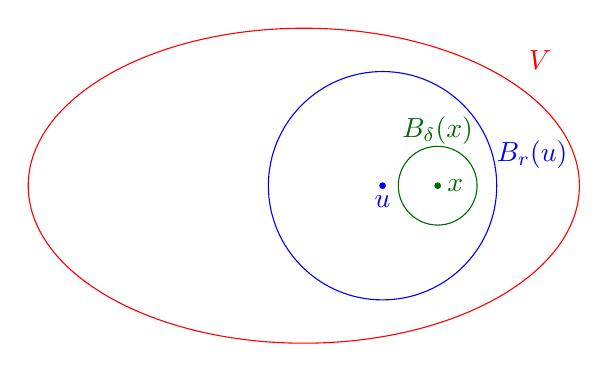
\begin{tikzpicture}
			\draw[red] (0,0) circle [x radius=3.5cm, y radius=2cm] ;
			\draw (3,1.6) node[red]{$V$};
			\draw [blue] (1,0) circle (1.45cm) ;
			\filldraw[blue] (1,0) circle (1pt) node[anchor=north]{$u$};
			\draw (2.9,0.4) node[blue]{$B_r(u)$};
			\draw [green!40!black] (1.7,0) circle (0.5cm) node [yshift=0.7cm]{$B_{\delta}(x)$} ;
			\filldraw[green!40!black] (1.7,0) circle (1pt) node[anchor=west]{$x$};
		\end{tikzpicture}
	\end{center}

	Given $x\in B_r(u)\subset V$, we want $\delta>0$ such that $x\in B_{\delta} (x)\subset B_r(u)\subset V$. Let $d=d(u,x)$. Choose $\delta $ such that $d+\delta<r$ (e.g. $\delta<\frac{r-d}{2}$)

	If $y\in B_{\delta}(x)$ we will be done by showing that $d(u,y)<r$ but $$d(u,y)\leq d(u,x)+d(x,y)<d+\delta<r$$
\end{myproof}

\cor{}{By the result of the proof, we can then show...}
\mlenma{}{Suppose $\vec{v_1}, \dots, \vec{v_n} \in \RR[n]$ is subspace of $\RR^n$.}
\mprop{}{$1 + 1 = 2$.}

\section{Random}
\dfn{Normed Linear Space and Norm $\boldsymbol{\|\cdot\|}$}{Let $V$ be a vector space over $\bbR$ (or $\bbC$). A norm on $V$ is function $\|\cdot\|\ V\to \bbR_{\geq 0}$ satisfying \begin{enumerate}[label=\bfseries\tiny\protect\circled{\small\arabic*}]
		\item \label{n:1}$\|x\|=0 \iff x=0$ $\forall$ $x\in V$
		\item \label{n:2}	$\|\lambda x\|=|\lambda|\|x\|$ $\forall$ $\lambda\in\bbR$(or $\bbC$), $x\in V$
		\item \label{n:3} $\|x+y\| \leq \|x\|+\|y\|$ $\forall$ $x,y\in V$ (Triangle Inequality/Subadditivity)
	\end{enumerate}And $V$ is called a normed linear space.

	$\bullet $ Same definition works with $V$ a vector space over $\bbC$ (again $\|\cdot\|\to\bbR_{\geq 0}$) where \ref{n:2} becomes $\|\lambda x\|=|\lambda|\|x\|$ $\forall$ $\lambda\in\bbC$, $x\in V$, where for $\lambda=a+ib$, $|\lambda|=\sqrt{a^2+b^2}$ }


\ex{$\bs{p-}$Norm}{\label{pnorm}$V={\bbR}^m$, $p\in\bbR_{\geq 0}$. Define for $x=(x_1,x_2,\cdots,x_m)\in\bbR^m$ $$\|x\|_p=\Big(|x_1|^p+|x_2|^p+\cdots+|x_m|^p\Big)^{\frac1p}$$(In school $p=2$)}
\textbf{Special Case $\bs{p=1}$}: $\|x\|_1=|x_1|+|x_2|+\cdots+|x_m|$ is clearly a norm by usual triangle inequality. \par
\textbf{Special Case $\bs{p\to\infty\ (\bbR^m$ with $\|\cdot\|_{\infty})}$}: $\|x\|_{\infty}=\max\{|x_1|,|x_2|,\cdots,|x_m|\}$\\
For $m=1$ these $p-$norms are nothing but $|x|$.
Now exercise
\qs{}{\label{exs1}Prove that triangle inequality is true if $p\geq 1$ for $p-$norms. (What goes wrong for $p<1$ ?)}
\sol{\textbf{For Property \ref{n:3} for norm-2}	\subsubsection*{\textbf{When field is $\bbR:$}} We have to show\begin{align*}
		         & \sum_i(x_i+y_i)^2\leq \left(\sqrt{\sum_ix_i^2} +\sqrt{\sum_iy_i^2}\right)^2                                       \\
		\implies & \sum_i (x_i^2+2x_iy_i+y_i^2)\leq \sum_ix_i^2+2\sqrt{\left[\sum_ix_i^2\right]\left[\sum_iy_i^2\right]}+\sum_iy_i^2 \\
		\implies & \left[\sum_ix_iy_i\right]^2\leq \left[\sum_ix_i^2\right]\left[\sum_iy_i^2\right]
	\end{align*}So in other words prove $\langle x,y\rangle^2 \leq \langle x,x\rangle\langle y,y\rangle$ where
	$$\langle x,y\rangle =\sum\limits_i x_iy_i$$

	\begin{note}
		\begin{itemize}
			\item $\|x\|^2=\langle x,x\rangle$
			\item $\langle x,y\rangle=\langle y,x\rangle$
			\item $\langle \cdot,\cdot\rangle$ is $\bbR-$linear in each slot i.e. \begin{align*}
				      \langle rx+x',y\rangle=r\langle x,y\rangle+\langle x',y\rangle	\text{ and similarly for second slot}
			      \end{align*}Here in $\langle x,y\rangle$ $x$ is in first slot and $y$ is in second slot.
		\end{itemize}
	\end{note}Now the statement is just the Cauchy-Schwartz Inequality. For proof $$\langle x,y\rangle^2\leq \langle x,x\rangle\langle y,y\rangle $$ expand everything of $\langle x-\lambda y,x-\lambda y\rangle$ which is going to give a quadratic equation in variable $\lambda $ \begin{align*}
		\langle x-\lambda y,x-\lambda y\rangle & =\langle x,x-\lambda y\rangle-\lambda\langle y,x-\lambda y\rangle                                       \\
		                                       & =\langle x ,x\rangle -\lambda\langle x,y\rangle -\lambda\langle y,x\rangle +\lambda^2\langle y,y\rangle \\
		                                       & =\langle x,x\rangle -2\lambda\langle x,y\rangle+\lambda^2\langle y,y\rangle
	\end{align*}Now unless $x=\lambda y$ we have $\langle x-\lambda y,x-\lambda y\rangle>0$ Hence the quadratic equation has no root therefore the discriminant is greater than zero.

	\subsubsection*{\textbf{When field is $\bbC:$}}Modify the definition by $$\langle x,y\rangle=\sum_i\overline{x_i}y_i$$Then we still have $\langle x,x\rangle\geq 0$}

\section{Algorithms}
\begin{algorithm}[H]
	\KwIn{This is some input}
	\KwOut{This is some output}
	\SetAlgoLined
	\SetNoFillComment
	\tcc{This is a comment}
	\vspace{3mm}
	some code here\;
	$x \leftarrow 0$\;
	$y \leftarrow 0$\;
	\uIf{$ x > 5$} {
		x is greater than 5 \tcp*{This is also a comment}
	}
	\Else {
		x is less than or equal to 5\;
	}
	\ForEach{y in 0..5} {
		$y \leftarrow y + 1$\;
	}
	\For{$y$ in $0..5$} {
		$y \leftarrow y - 1$\;
	}
	\While{$x > 5$} {
		$x \leftarrow x - 1$\;
	}
	\Return Return something here\;
	\caption{what}
\end{algorithm}

\end{document}
